\documentclass[a4paper,10pt]{article}


\usepackage{t1enc}
\usepackage{linguex}
\usepackage{harvard}
\usepackage{graphicx}
\usepackage{amsmath}
\usepackage{amssymb}
\usepackage{graphicx}
\usepackage{tikz}
\usetikzlibrary{arrows,automata}
\usepackage{subfigure}
\usepackage{qtree}
%\usepackage{hyperref}




\bibliographystyle{diss}

%opening
\title{Results K2 (Target Conditions)}
\author{}



\newtheorem{hypothese}{Hypothesis}
\newtheorem{Def}{Definition}
\newtheorem{Prop}{Proposition}
\newtheorem{Example}{Example}

\begin{document}

\maketitle

\begin{abstract}

\end{abstract}

\section{Design}

\paragraph{General Idea:} In order to test whether local implicatures are possible, we seeked for a way to unambiguously map responses from a picture verification task to the alternative readings of AS- and ES-sentences. In addition, we wanted to minimize effects of any graphical differences between the picture materials. To achieve this we designed an experiment employing a modified version of picture verification, namely the incremental verification task (IVT, see Conroy). We will now describe the design step by step.

Consider the AS-sentence in \Next. With respect to figure \ref{fig:exseqAS3} the local reading is false, while the global and literal reading is true. Now, we made use of the following fact. If we cover up certain edges in the graph as in Figure \ref{fig:exseqAS2} the literal and global reading is still true, but the local reading is not decidable (assuming we haven't seen the whole graph, yet). By covering even a greater part of the graph, we can go one step further. In Figure \ref{fig:exseqAS1} the literal reading is true, while the local and global reading cannot be decided, yet. Now, consider the following task. Participants are asked to read sentence \Next and then uncover a graph step by step until they feel able to give a truth value judgment. In this task the participant has three options at each step: (1) demand more information (2) judge the sentence as true (3) judge the sentence as false. Presenting a sequence like Figure \ref{fig:exseqAS}, we obtain the desired mapping between judgments and readings. This mapping is illustrated in Figure \ref{fig:mappingAS}.


For the ES-sentences, the idea is similar. With respect to the sentence in \NNext we obtain an unambiguous mapping between truth values and readings with respect to the sequence in \ref{fig:exseqES}. This is illustrated in Figure \ref{fig:mappingES}. There are two differences to the previous case. Firstly, the order of readings that can be identified in the sequence differs. At the first step the global reading can be judged. Then the literal and, finally, the local reading can be judged. Secondly, the readings correspond to different truth values. Global and literal readings correspond to negative truth values, while local reading require positive judgments.  

\exg. \label{ex:as}{\bf Jeder} Brief ist mit {\bf einigen} seiner Dreiecke verbunden.\\
Every Letter is with some its triangles connected.\\
Every letter is connected to some of its triangles.

\exg. \label{ex:es}{\bf Genau} eine Glocke ist mit {\bf einigen} ihrer Halbkreise verbunden.\\
Exactly one Letter is with some its semicircles connected.\\
Exactly one letter is connected to some of its semicircless.

\begin{figure}[ht]
	\centering
	\subfigure[Step 3]{ 
		\fbox{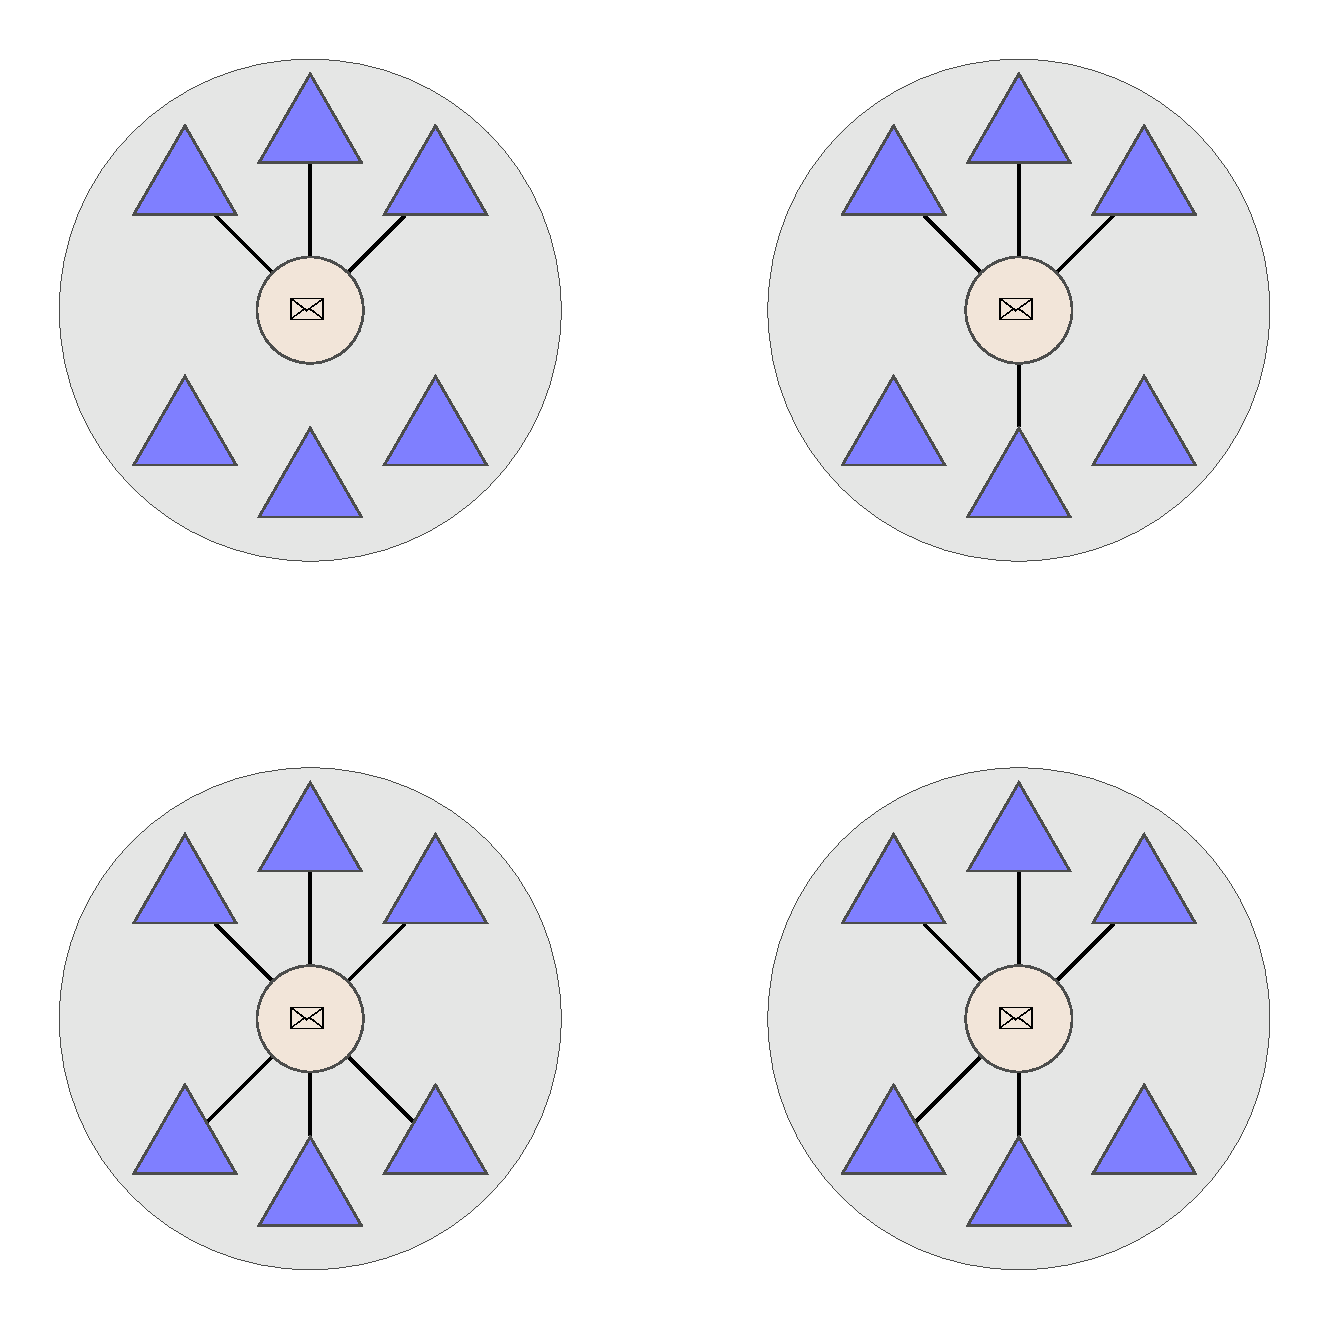
\includegraphics[width=3cm]{ae_7_v_l.pdf}}
	    \label{fig:exseqAS3}
	}
	\subfigure[Step 2]{
		\fbox{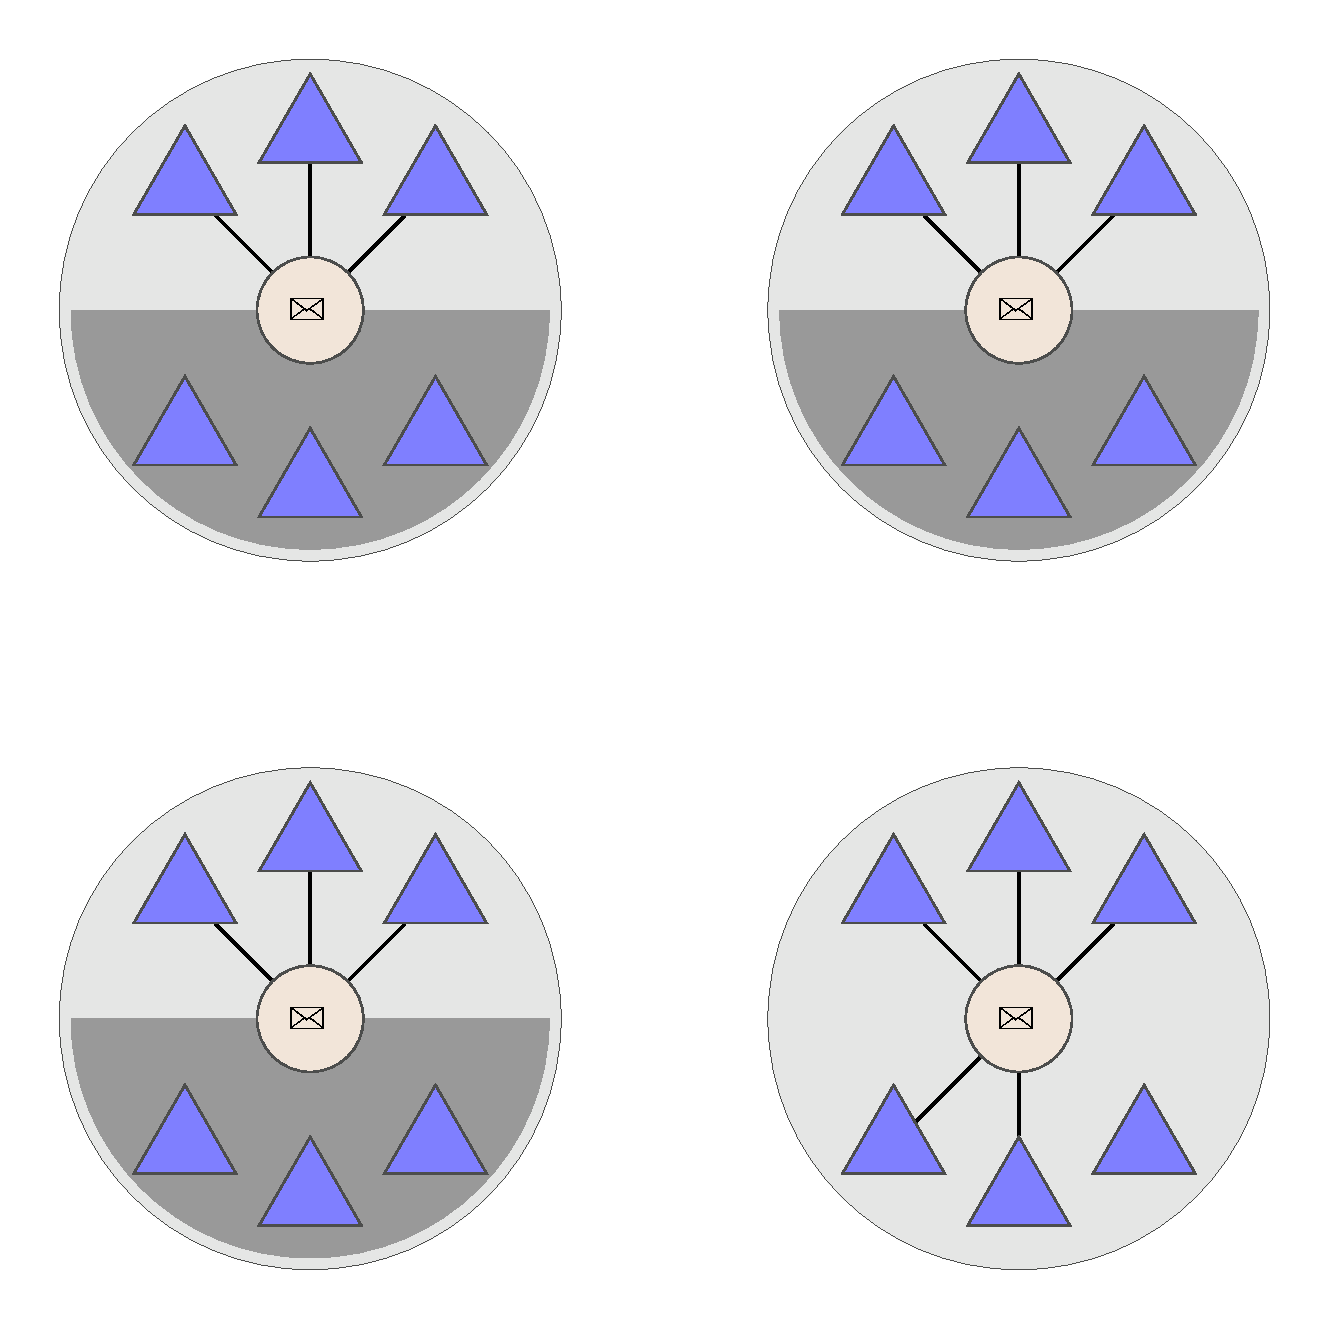
\includegraphics[width=3cm]{ae_5_v_l.pdf}}
	    \label{fig:exseqAS2}
	}
	\subfigure[Step 1]{ 
		\fbox{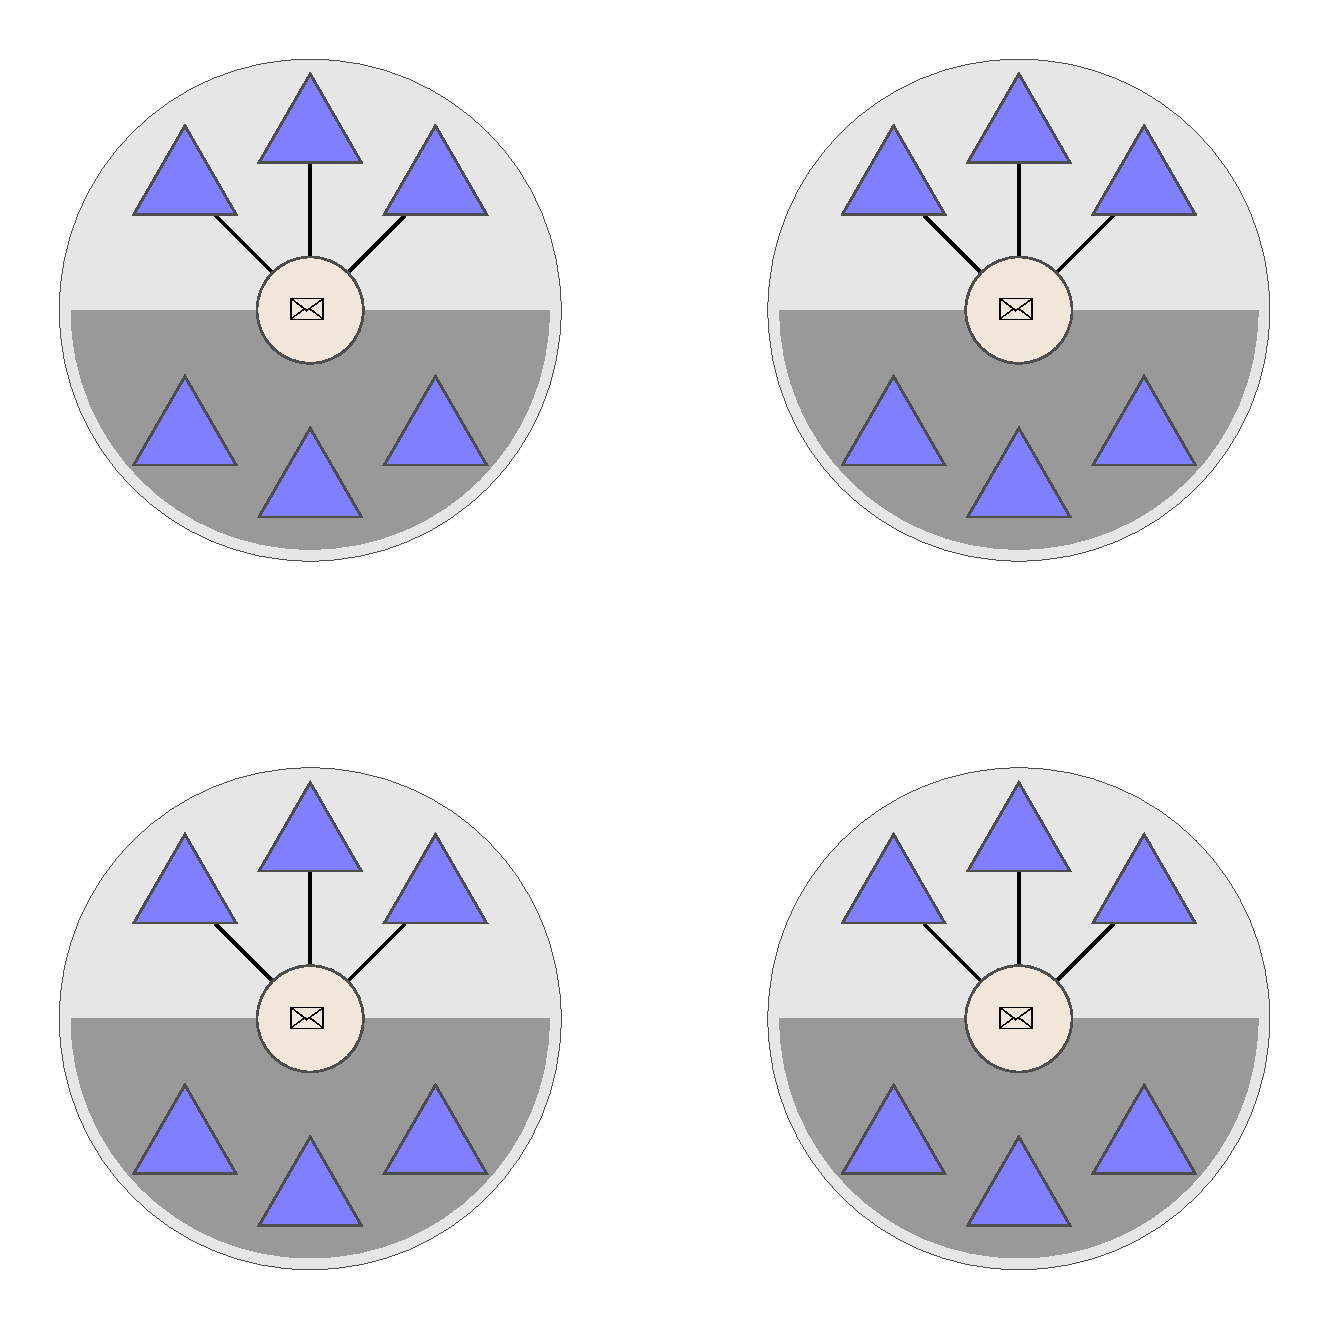
\includegraphics[width=3cm]{ae_3_v_l.pdf}}
	    \label{fig:exseqAS1}
	}
	\caption[]{Example sequence for AS-sentences}
	\label{fig:exseqAS}
\end{figure}

\begin{figure}[ht]
	\centering
	\subfigure[Step 3]{ 
		\fbox{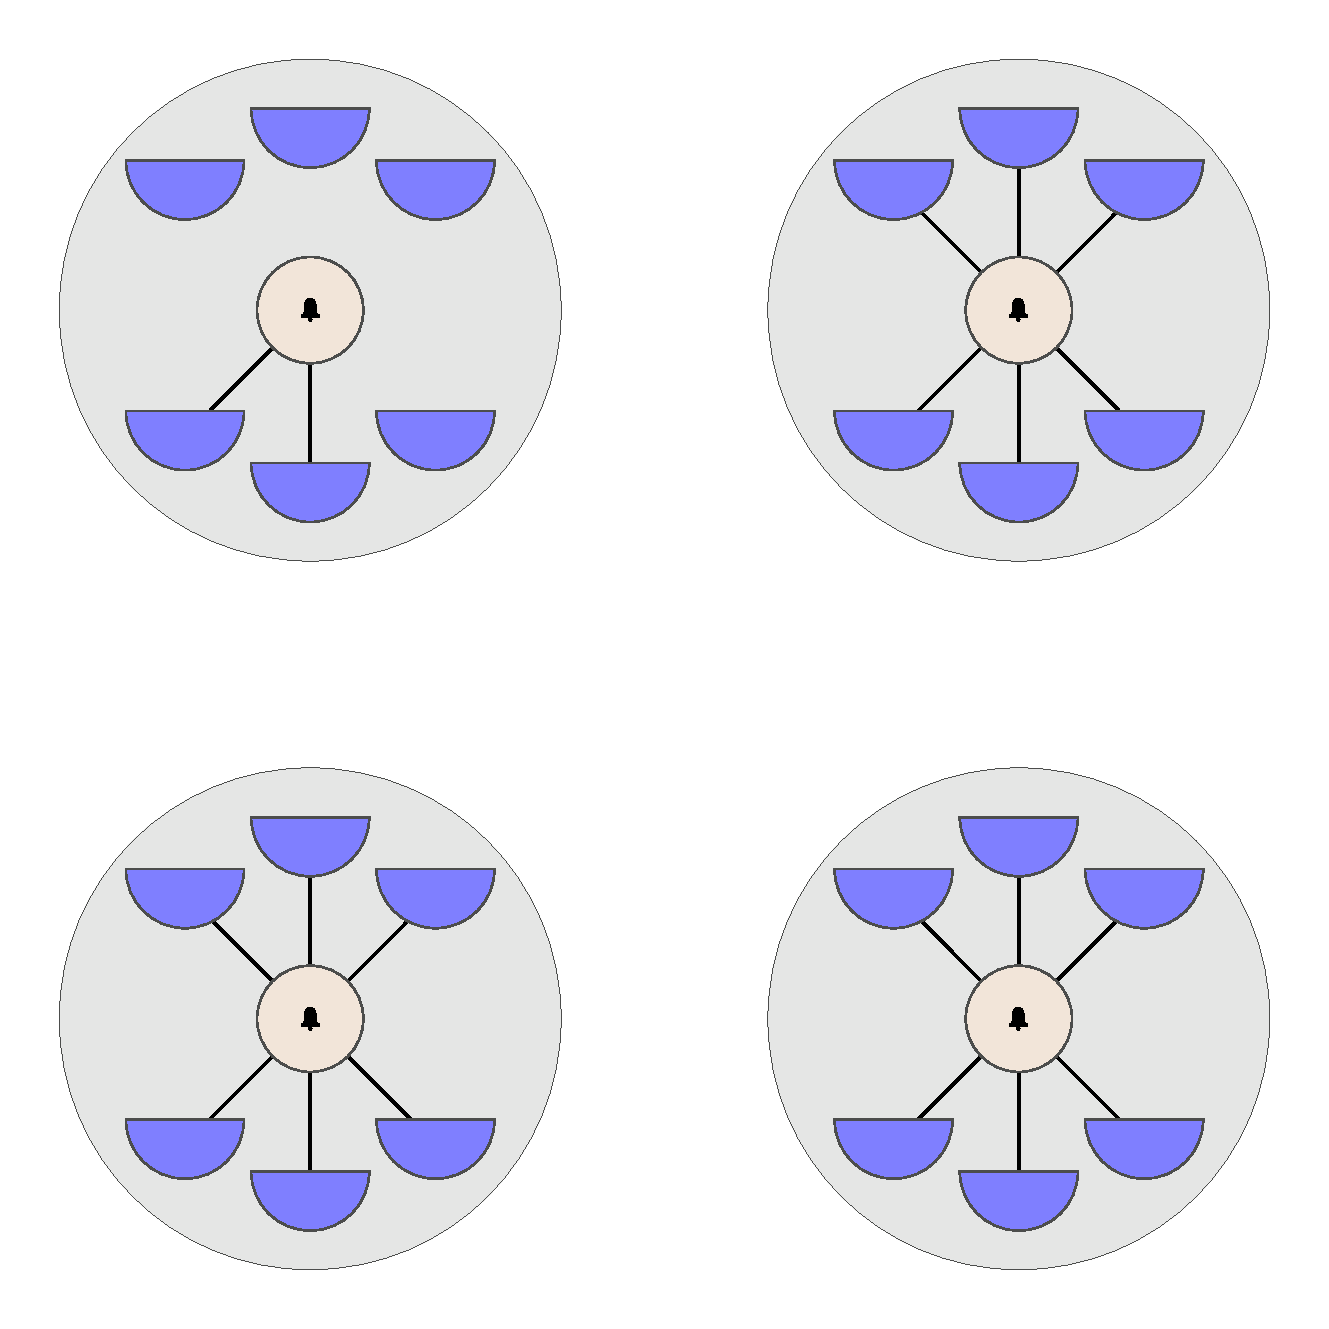
\includegraphics[width=3cm]{ge_6_v_l.pdf}}
	    \label{fig:subfig1}
	}
	\subfigure[Step 2]{
		\fbox{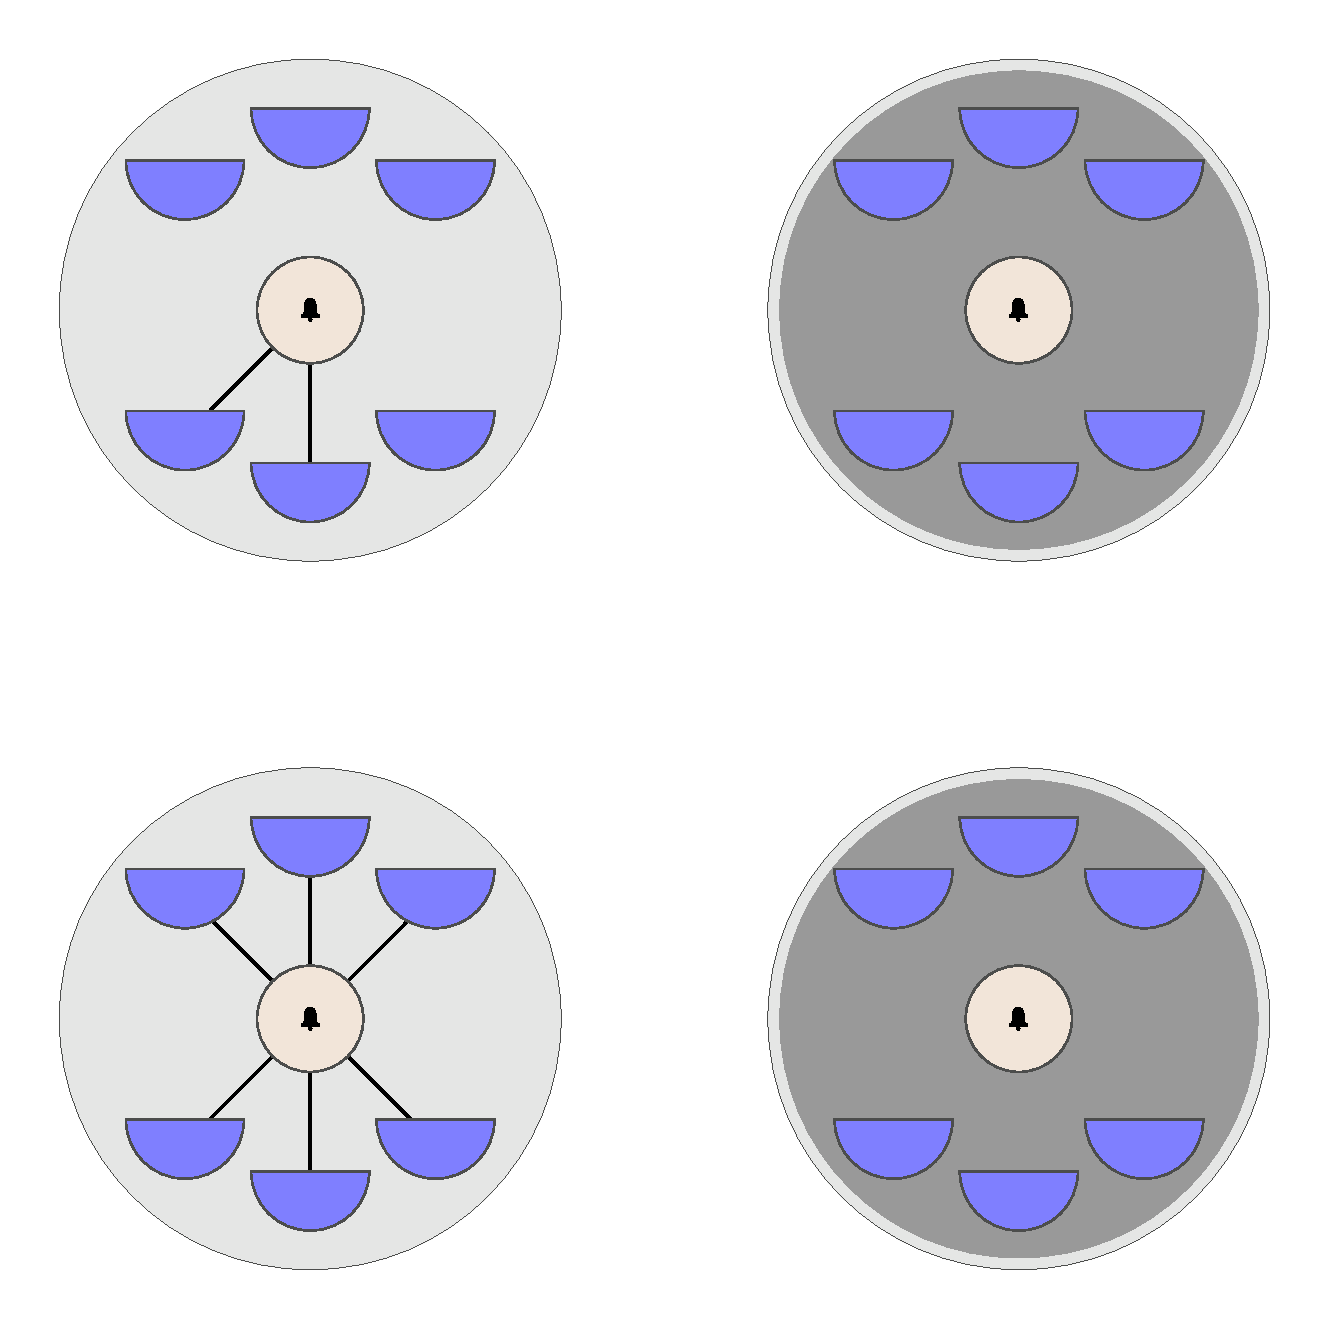
\includegraphics[width=3cm]{ge_4_v_l.pdf}}
	    \label{fig:subfig2}
	}
	\subfigure[Step 1]{ 
		\fbox{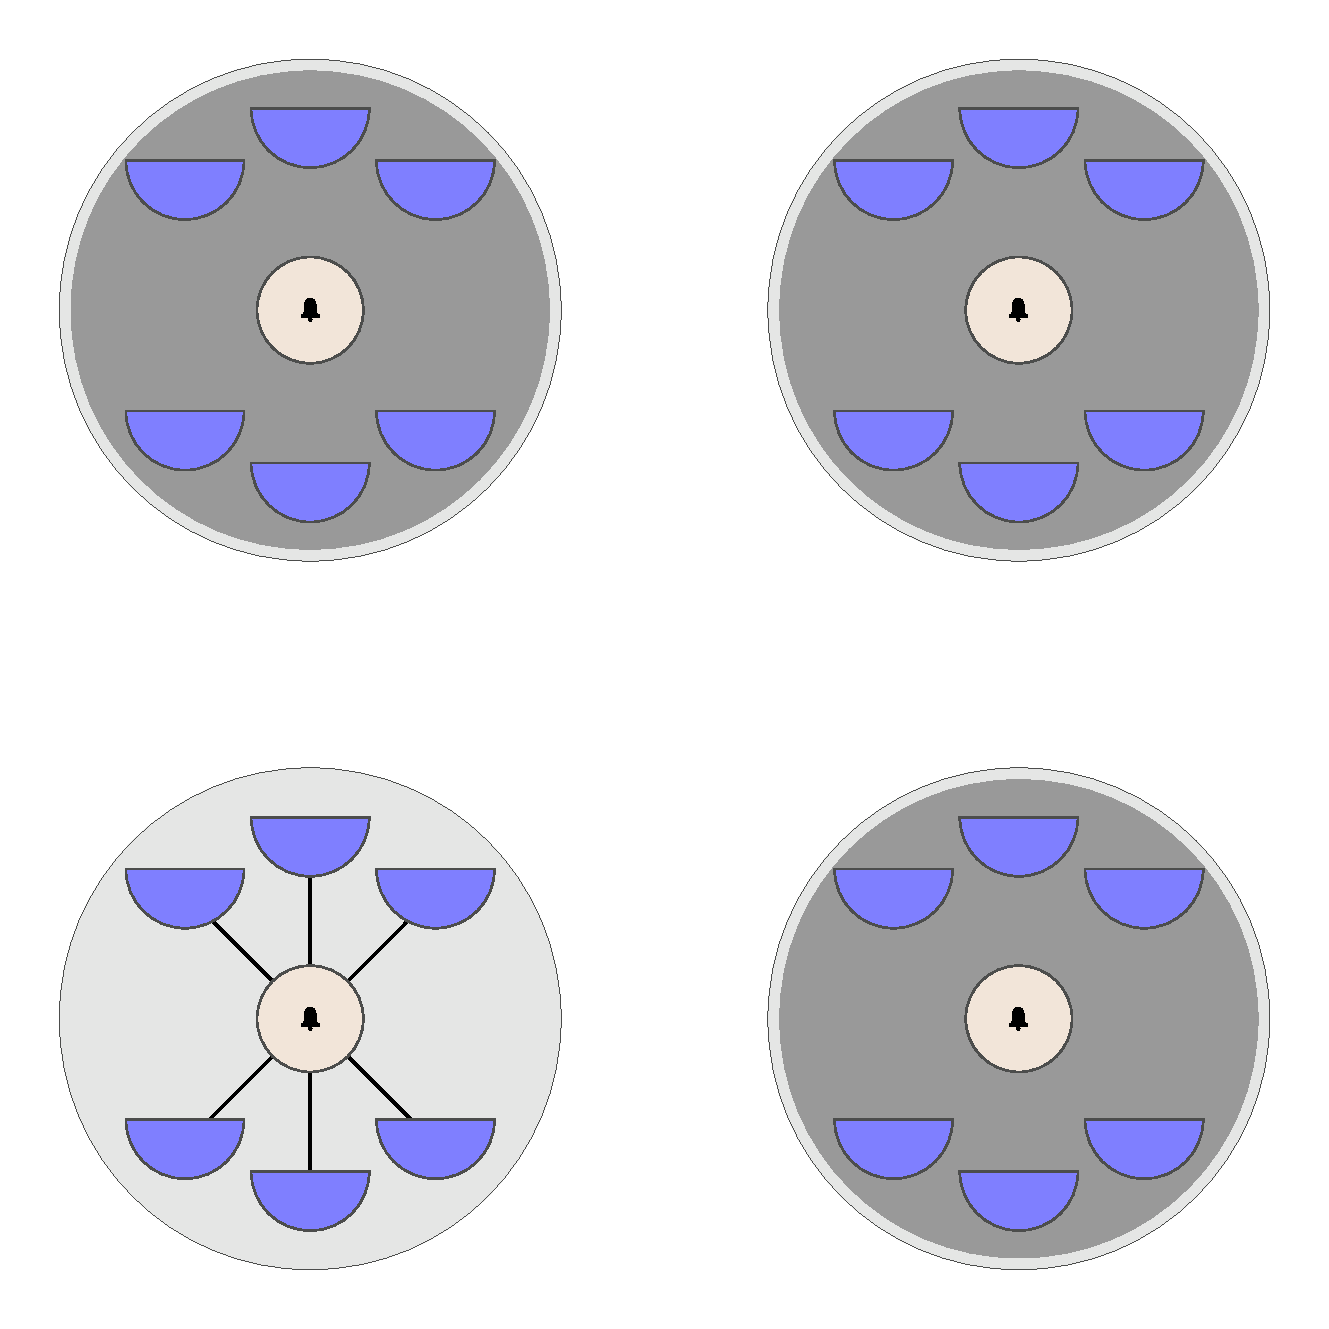
\includegraphics[width=3cm]{ge_3_v_l.pdf}}
	    \label{fig:subfig1}
	}
	\caption[]{Example sequence for AS-sentences}
	\label{fig:exseqES}
\end{figure}






\begin{figure}[ht]
	\centering
	\subfigure[AS-Sentences]{ 
\begin{tabular}{cccc}
&more info&true&false\\
\hline
Step 1&?&literal&?\\
Step 2&?&global&?\\
Step 3&?&?&local\\
\hline
\end{tabular}

	    \label{fig:mappingAS}
	}
	\subfigure[ES-Sentences]{
\begin{tabular}{cccc}
&more info&true&false\\
\hline
Step 1&?&literal&?\\
Step 2&?&global&?\\
Step 3&?&?&local\\
\hline
\end{tabular}
	    \label{fig:mappingES}
	}
	\caption{Mapping from truth values to readings}
	\label{fig:subfigureExample}
	\end{figure}


In addition to the unambiguous mapping from readings to truth values, we think that the present design minimizes graphical effects because there is no comparison between different pictures. The distribution of responses found in previous studies could in part be explained by differences in typicality of the pictures with respect to the possible readings (see van Tiel). In the present case this kind of reasoning would have to be extended to the typicalilty of parts of pictures. On intuitive grounds, we take this kind of reasoning to be implausible. We will now shortly discuss how graphical properties might still affect judgments in the worst case. In the first step of the AS-condition local and global readings cannot be judged, yet. Therefore, graphical properties should not affect judgments if participants have one of these readings in mind. If participants have a literal reading in mind, the worst case scenario is that they refrain from judging the sentence as true at this point due to some, eg. atypical, graphical property of the picture. The situation is similar at the second step. The local reading is still not decidable. Therefore, graphical properties should not play a role if participants have a local reading in mind. A positive judgment might, however, be a delayed judgment of a literal reading. Again, the worst case scenario for our purpose is that participants refrain from answering because of graphical properties. At the last step the local reading requires a negative judgment. Now, we could obtain delayed negative responses from literal or global readings because the graph as a whole is, e.g., logically true but atypical with respect to these readings. These kinds of judgments would be indistinguishable from local responses. Note, however, that we have no reason to believe that typicality has large effects,  because, given the results from van Tiel, the picture as a whole is expected to be one of the more typical situations for AS-sentences. Still, we cannot exclude the possibility that graphical properties of the pictures might have the described effect. In the ES-conditions this type of effect is, however, entirely impossible since the  literal and global reading is plainly false given the initial parts as well as the whole graph. Summing up, in the worst case, which we consider implausible, graphical effects might lead to an enhanced number of local responses in the AS- as compared to the ES-condition. We have to keep this possibility in mind. We want to stress, however, that the design presented here improves on previous studies with respect to possible graphical effects.

\paragraph{Testing Effects of accentuation:} It has been claimed that local readings only emerge in the case of special accentuation of the the scalar item under consideration (REFERENCES). Further, it is generally assumed that the required type of accentuation is a pitch accent (REFS). To test for this possibility we decided to present the sentences  (eg., \LLast and \Last) auditively in two versions each. In the accented version a pitch accent was palced on {\it einige}. The second version had neutral prosody. If accentuation is the driving force for local readings, we would expect a higher proportion of local readings in the former than in the latter version of the sentences.

\paragraph{Controlling Response biases:} In order to control for response biases that are independent of the sentence meaning, but only depend on the experimental procedure or on the picture materials, we generated a set of control conditions. For all three readings in the AS- and ES-conditions we constructed one unambiguous control sentence requiring the same type of response at the same point in the sequence. We used sentences as in \Next and \NNext. Example \Next[a] requires the same response as the AS-sentence in \ref{ex:as} under its literal reading, \Next[b] corresponds to the AS-sentence under its global reading and \Next[c] corresponds to the local reading. With regard to the ES-sentences, controls like \NNext[a] correspond to the global reading, \NNext[b] to the literal and \NNext[c] to the local reading.  If, independently from sentence meaning, there was any bias to respond in a certain way at any point in the sequences this should affect the control sentences to the same degree as it affects the target conditions.

\ex. \ag. Alle W\"urfel sind mit mindestens drei ihrer Dreiecke verbunden.\\
All dice are with at-least three their triangles connected.\\
All dice are connected to at least three of their triangles. 
\bg. Mindestens ein Brief ist mit genau f\"unf seiner Quadrate verbunden.\\
At-least one letter is with exactly five his squares connected.\\
At least one letter is connected with exactly five of his squares. 
\bg. Jeder Brief ist mit mindestens vier seiner Quadrate verbunden.\\
Every letter is with at-least four his squares connected.\\
Every letter is connected to at least four of its squares.


\ex. \ag. Alle Glocken sind mit weniger als vier ihrer Halbkreise verbunden. \\
All bells are with fewer than four their semicircles connected.\\
All bells are connected with fewer than four of their semicircles.  
\bg. Alle Glocken sind mit allen ihren Halbkreisen verbunden.\\
All bells are with all their semicircles connected.\\
All bells are connected to all of their semicircles. 
\bg. Mindestens drei Glocken sind mit allen ihren Halbkreisen verbunden.\\
At-least three bells are with all  their semicircles connected.\\
At least three bells are connectd with all of their semicircles.



\paragraph{Controlling ambiguity resolution} In order to confidently interpret the results obtained in the described IVT experiment, we need to know certain facts about how participants deal with amiguous sentences in the IVT (disccussion of Conroy's study). To ivestigate this we used a second type of control conditions. In particular, we tested (1) whether the order in which readings can be judged affects preferences for ambiguous sentences and (2) whether prosodic information can, in principle, shift reading preferences in the present task. To this end, we used ambiguous sentences of the type in \Next. In the literature (REFS) two readings are reported for sentences of this kind. Under the first reading the PP {\it with suns} modifies the complete conjunction {\it circles and squares}. This reading is called the high-attachment reading. Under the second, low-attachment, reading the PP only modifies the second conjunct, {\it squares}. Generally, the late closure reading is preferred over the early closure reading for sentences like \Next (REFS). Concerning presentation order of readings, it is crucial for our purpose that dispreferd readings are in principle detectable regardless of their position in the sequence. To test this we combined sentences like \Next with two kinds of sequences. In the first kind of sequence a partly uncovered graph like in figure \ref{fig:exec1} preceeds a graph like in figure \ref{fig:exec2}. Here, the high-attachment reading can be judged first. Under this reading we would expect a "no"-judgment on \ref{fig:exec1}. Under the low-attachment reading we would, in contrast, expect a "yes"-response on \ref{fig:exec2}. The order of presentation is reversed in the second kind of sequence which included pictures like \ref{fig:exlc1} folllowed by pictures like \ref{fig:exlc2}. Here, the low-attachment reading can be judged first requiring a "yes"-response on \ref{fig:exlc1}. The high-attachment reading can only be judged later in the sequence. When we reach \ref{fig:exlc2} a "no"-response is expected under a high-attachment reading. If presentation order does affect preferences, we would expect preferences to differ between the two types of sequences. 

\exg. Die Brief ist mit Kreisen und Vierecken mit Sonnen verbunden.\\
The letter is with circles and squares with suns connected.\\
The letter is connected with circles and squares with suns.

\begin{figure}[ht]
	\centering
	\subfigure[Step 1]{ 
		\fbox{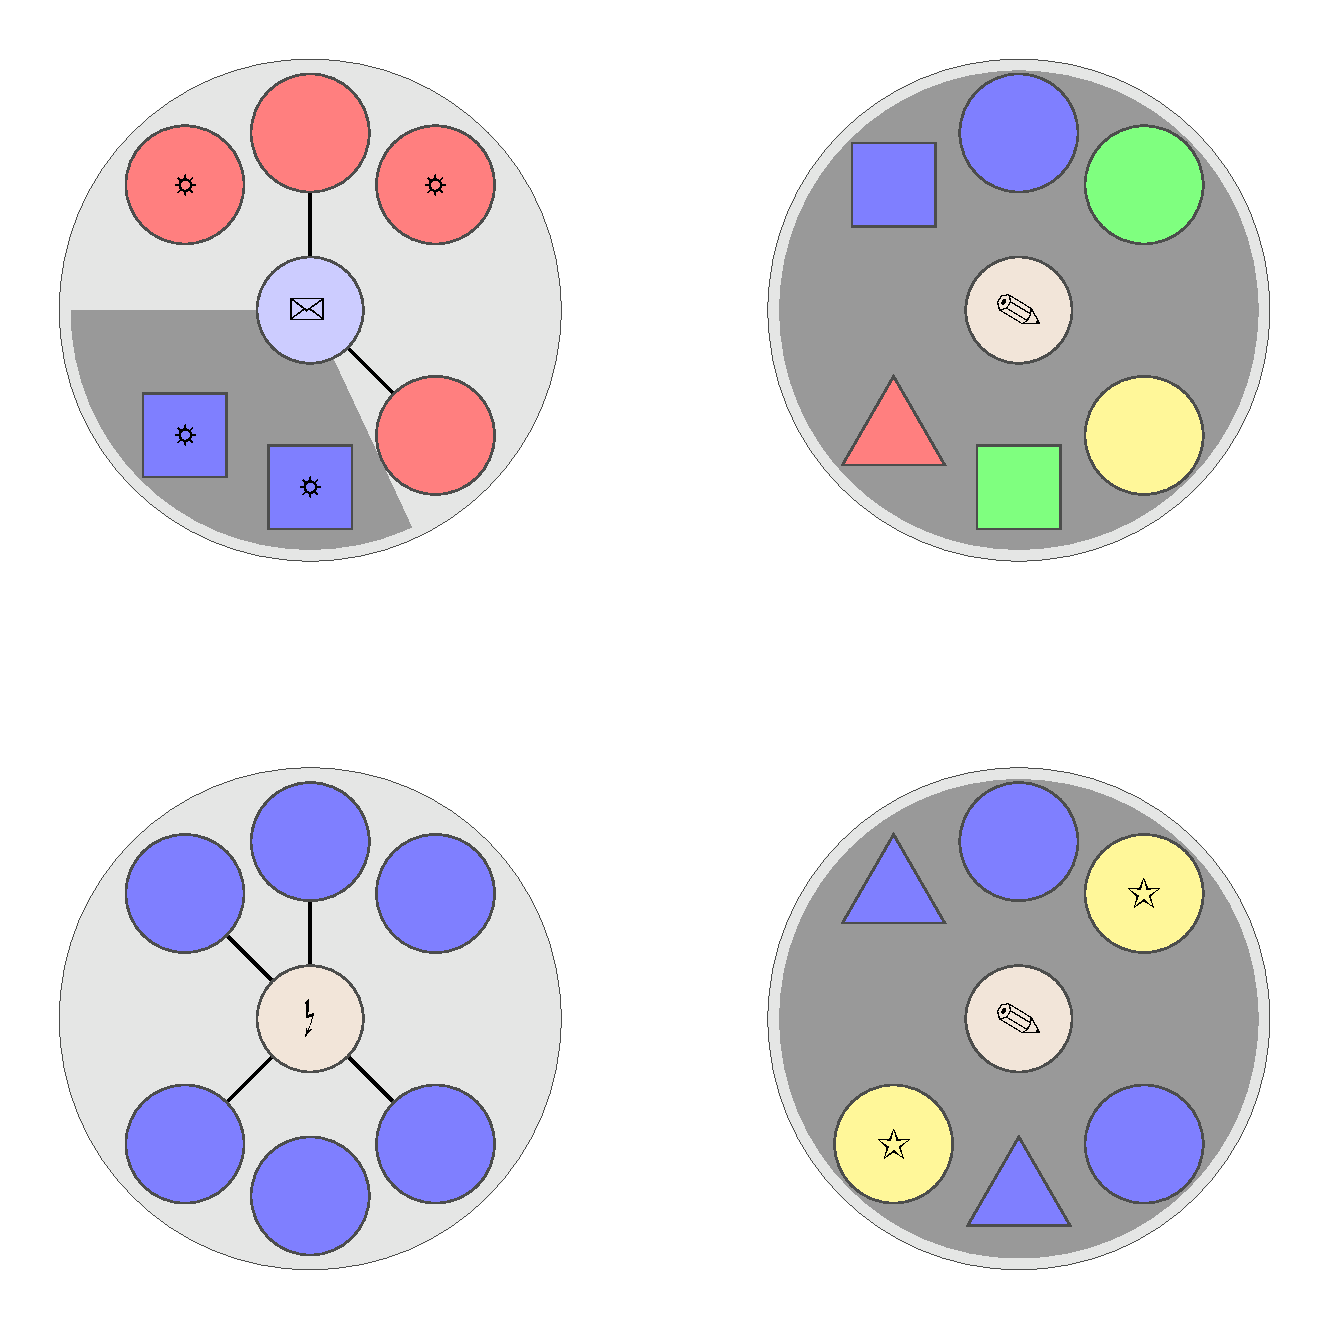
\includegraphics[width=3cm]{ec_01_3.pdf}}
	    \label{fig:exec1}
	}
	\subfigure[Step 2]{
		\fbox{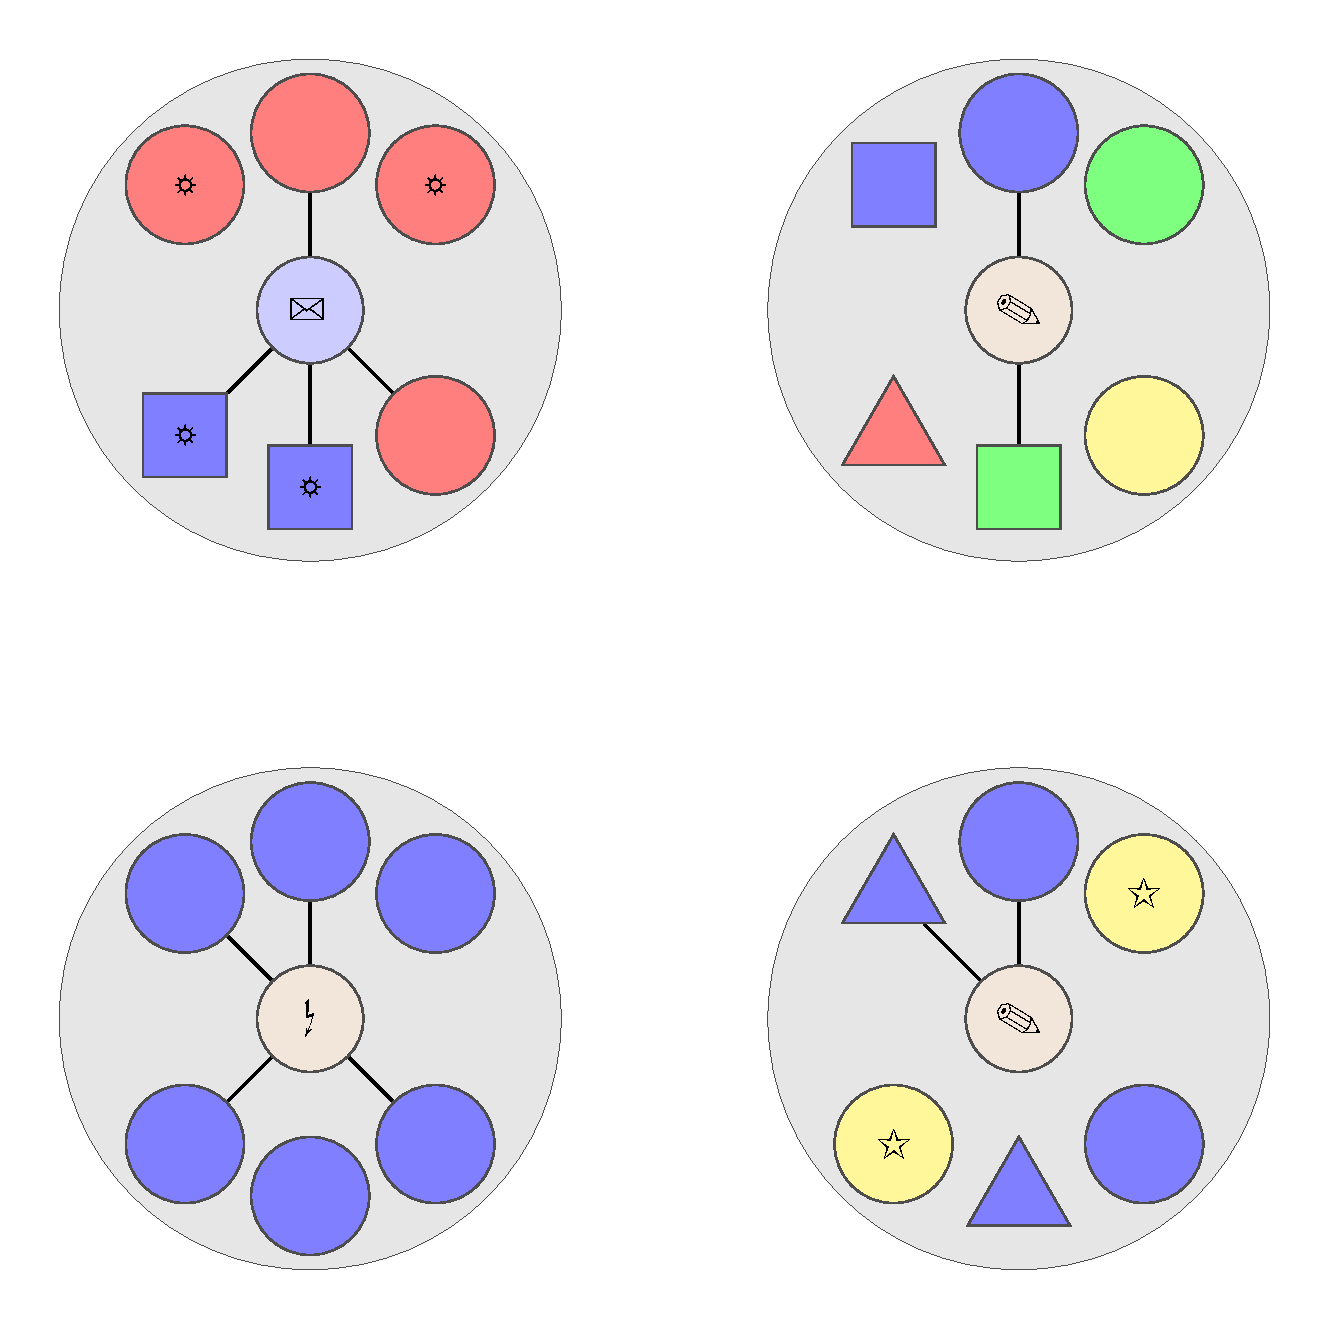
\includegraphics[width=3cm]{ec_01_5.pdf}}
	    \label{fig:exec2}
	}
	\caption[]{High-attachment first}
	\label{fig:exec}
\end{figure}

\begin{figure}[ht]
	\centering
	\subfigure[Step 1]{ 
		\fbox{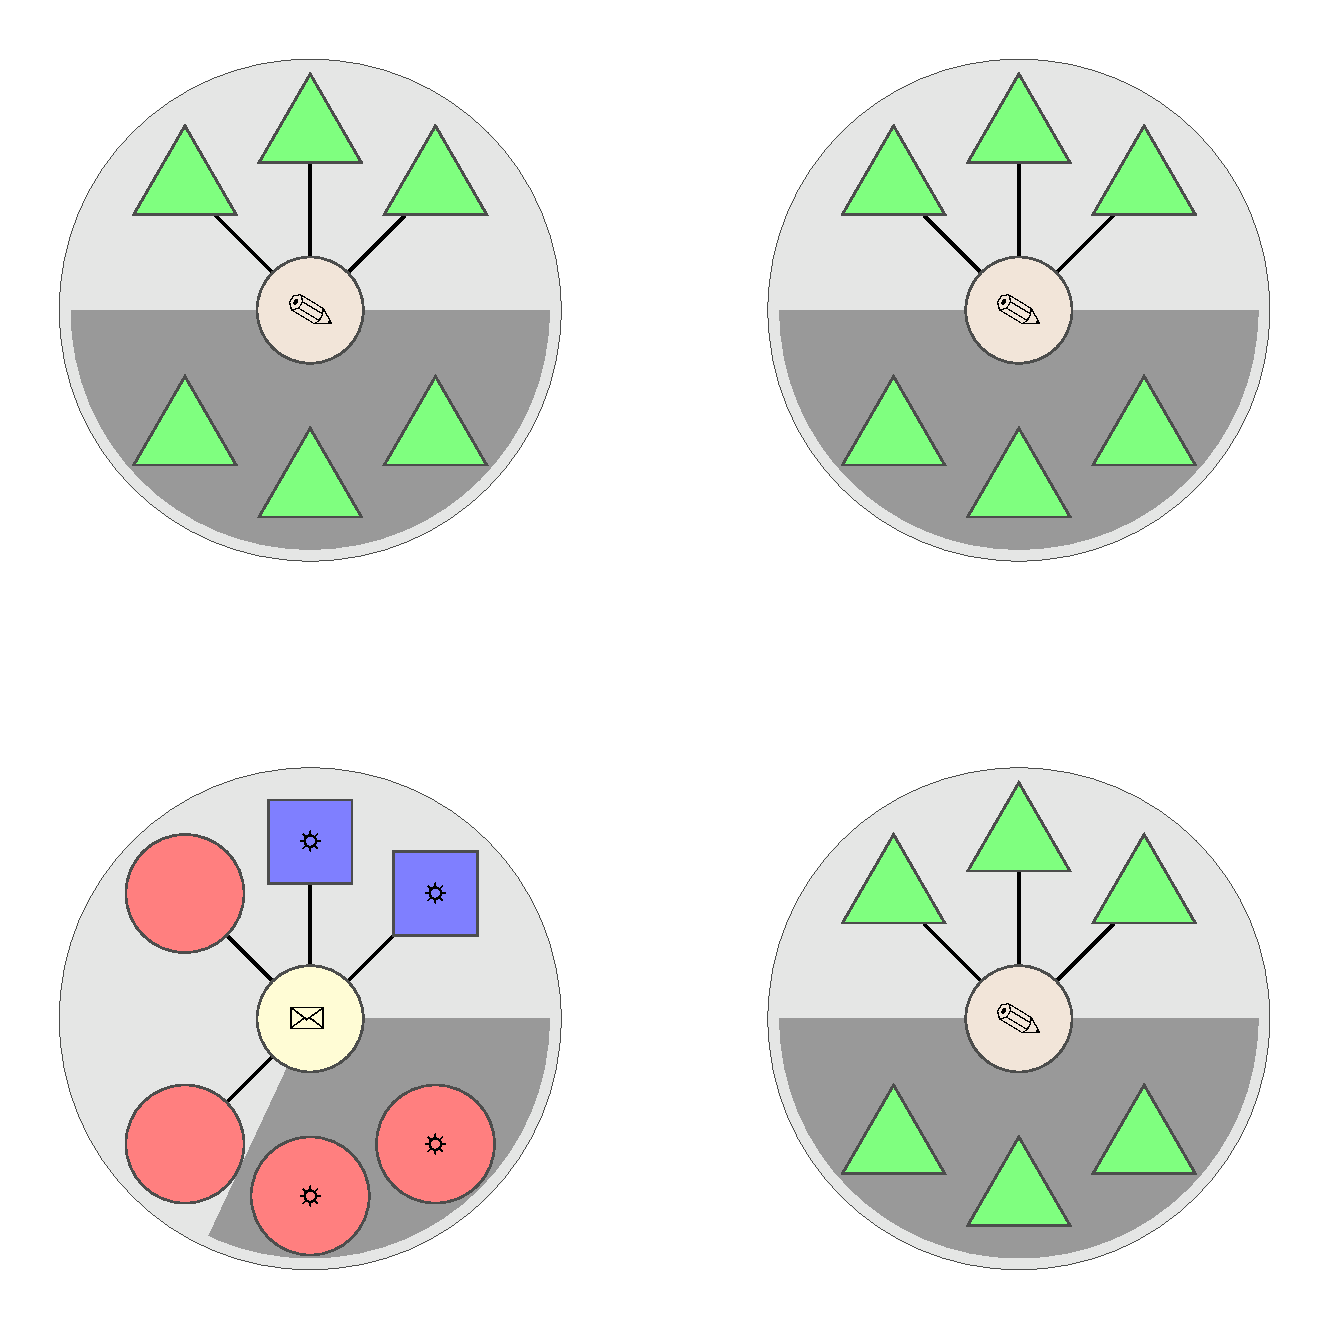
\includegraphics[width=3cm]{lc_01_3.pdf}}
	    \label{fig:exlc1}
	}
	\subfigure[Step 2]{
		\fbox{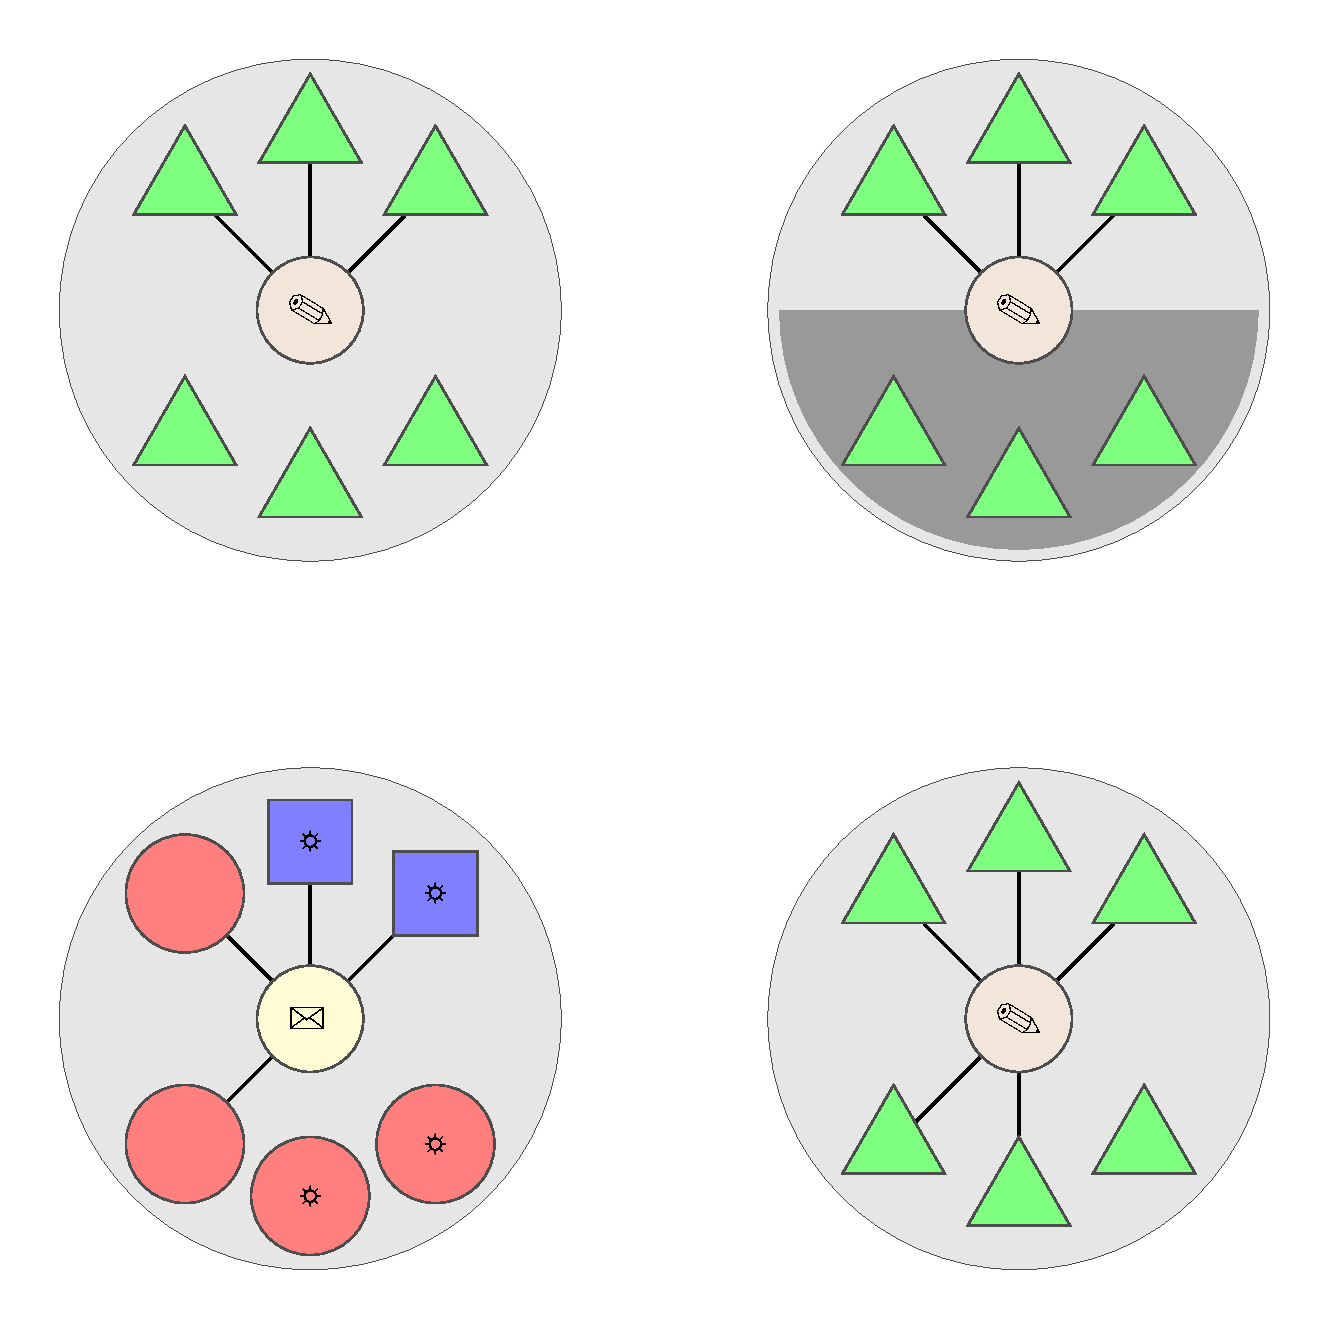
\includegraphics[width=3cm]{lc_01_6.pdf}}
	    \label{fig:exlc2}
	}
	\caption[]{Low-attachment first}
	\label{fig:exec}
\end{figure}

Concerning prosodic information, we wanted to make sure that differences in prosody may generally lead to a shift in interpretation preferences in the ITV task. Sentences like \Last are well suited to test this assumption since it is well-known that their interpretational preferences are sensitive to prosody. The most natural way to pronounce a sentence like \Last includes a prosodic phrase boundary between {\it squares} and {\it with}. This intonation pattern strongly corresponds to the high-attachment reading. If, instead, a prosodic phrase boundary after {\it circles} is present, the acceptance of the low-attachment reading is boosted. To test whether prosodic information is taken into account in the IVT we presented both types of prosodic structures expecting the described boost in acceptance for the low-attachment reading. In addition, we also included a neutral version containing no phrase marking whatsoever. This should receive intermediate acceptance rates. Further, we also presented unambiguous sentences corresponding to the early closure reading. As in the case of the AS- and ES-sentences the unambiguous counterparts  served as a baseline to control for response biases that are independent of sentence meaning.  

     


\bibliography{../../Literatur/tex/literatur}
\end{document}
 